\section{Results}

Phần này tổng hợp kết quả kiểm thử và xác nhận tính đúng đắn của các khối logic cốt lõi (RTSP message handling, Timer kiểm soát nhịp), đồng thời mô tả các hành vi runtime có thể quan sát được từ client UI và các thống kê có sẵn trong mã nguồn.

\subsection{Kết quả kiểm thử đơn vị (Unit Tests)}

Dự án cung cấp bộ kiểm thử trong \code{common/tests} cho hai thành phần có rủi ro lỗi cao: (1) xây dựng và phân tích RTSP message, (2) Timer điều phối thời gian. Các test được viết theo phong cách ``lightweight framework'' (assert + reporter) và có thể chạy độc lập với Qt.

\begin{table}[H]
\centering
\caption{Tổng hợp kết quả unit test ở tầng Common}
\label{tab:unit_tests}
\begin{tabular}{lrr}
\toprule
Test Suite & Số test & Kết quả \\
\midrule
\code{test\_rtsp\_message} & 15 & 15 passed, 0 failed \\
\code{test\_timer} & 13 & 13 passed, 0 failed \\
\bottomrule
\end{tabular}
\end{table}

Kết quả chạy test RTSPMessage thể hiện cả các kịch bản cơ bản lẫn round-trip (build rồi parse lại). Đoạn log dưới đây minh họa phần tổng kết của suite (trích nguyên văn từ output).

\begin{lstlisting}[language={}, caption={Output tổng kết của \texttt{test\_rtsp\_message}}, label={lst:rtsp_test_output}]
Total: 15 tests
Passed: 15
Failed: 0
\end{lstlisting}

Tương tự, Timer được kiểm tra với nhiều interval (25 FPS, 30 FPS, 60 FPS), kiểm tra drift (không sleep khi ``work time'' vượt interval), và stress test. Đoạn log tổng kết:

\begin{lstlisting}[language={}, caption={Output tổng kết của \texttt{test\_timer}}, label={lst:timer_test_output}]
Total: 13 tests
Passed: 13
Failed: 0
\end{lstlisting}

\subsection{Chỉ số runtime sẵn có ở Client}

Ngoài unit test, Client đã tích hợp các thống kê runtime cho RTP: số packet nhận, số packet ước lượng mất, tổng bytes, và phần trăm loss. Loss được tính bằng chênh lệch sequence; do đó thống kê phản ánh mất gói ``theo thứ tự'' (out-of-order có thể bị tính như lost nếu đến quá muộn hoặc bị bỏ qua ở Reassembler tùy kịch bản).

\begin{lstlisting}[language=C++, caption={Công thức phần trăm mất gói RTP}, label={lst:loss_formula}]
double RTPReceiver::getPacketLossPercentage() const {
    uint64_t total = packetReceived_ + packetLost_;
    if (total == 0) return 0.0;
    return (static_cast<double>(packetLost_) * 100.0) / static_cast<double>(total);
}
\end{lstlisting}

\subsection{Hành vi buffer và prebuffer quan sát từ UI}

UI triển khai hai cơ chế nhằm tối ưu trải nghiệm: (1) prebuffer trước khi phát, (2) điều chỉnh nhịp render theo mức buffer. Prebuffer được kích hoạt khi bắt đầu PLAY hoặc khi xảy ra ``rebuffering'' do buffer cạn; điều này làm tăng độ ổn định, đổi lại là tăng độ trễ đầu phát.

\begin{table}[H]
\centering
\caption{Các tham số buffer quan trọng và ý nghĩa vận hành}
\label{tab:buffer_params}
\begin{tabular}{lll}
\toprule
Tham số & Vị trí & Ý nghĩa \\
\midrule
\code{PREBUFFER\_FRAMES} & \code{ClientUI} & Số frame cần tích lũy trước khi bắt đầu render \\
\code{LOW\_BUFFER\_THRESHOLD} & \code{ClientUI} & Ngưỡng cảnh báo buffer thấp và tăng interval render \\
\code{MAX\_PAYLOAD\_SIZE} & \code{RTPPacket} & Giới hạn payload/packet để tránh IP fragmentation \\
\bottomrule
\end{tabular}
\end{table}

\begin{lstlisting}[language=C++, caption={UI chuyển sang trạng thái ``Buffering'' khi buffer chưa đủ}, label={lst:ui_buffering_state}]
statusLabel_->setText(QString("Buffering... %1/%2 frames (%3%)")
    .arg(bufferSize)
    .arg(PREBUFFER_FRAMES)
    .arg(percentage, 0, 'f', 1));
\end{lstlisting}

\subsection{Hướng dẫn triển khai và tái lập kết quả}

\subsubsection{Thiết lập dự án thông qua \code{setup.py}}

Để đơn giản hóa quy trình triển khai trên các nền tảng khác nhau, dự án cung cấp script tự động hóa \code{setup.py} thực hiện toàn bộ các bước từ kiểm tra phụ thuộc đến biên dịch mã nguồn.

\paragraph{Quy trình tự động}

Script \code{setup.py} được thiết kế để hoạt động trên Linux, Windows (MSYS2), và macOS. Khi chạy, script sẽ:

\paragraph*{Phát hiện hệ điều hành}: Sử dụng \code{platform.system()} để xác định môi trường thực thi
\textbf{Kiểm tra Qt6}: Tìm kiếm Qt6 qua các phương pháp:
    \begin{itemize}
        \item Kiểm tra \code{qmake6} trong PATH
        \item Thực hiện CMake find\_package
        \item Tìm kiếm trong đường dẫn cài đặt phổ biến (MSYS2 MinGW64, Homebrew, v.v.)
    \end{itemize}
\paragraph*{Hướng dẫn cài đặt Qt6}: Nếu không tìm thấy, hiển thị hướng dẫn chi tiết theo từng nền tảng
\paragraph*{Cấu hình CMake}: Tự động thiết lập \code{CMAKE\_PREFIX\_PATH} và generator phù hợp (Make/Ninja)
\paragraph*{Biên dịch song song}: Sử dụng \code{make -j} hoặc \code{ninja} với tất cả các lõi CPU
\paragraph*{Hiển thị hướng dẫn sử dụng}: In ra cú pháp chạy server/client với ví dụ cụ thể

\paragraph*{Cách sử dụng}
\noindent

\begin{lstlisting}[language=bash, caption={Chạy script setup tự động}, label={lst:setup_script}]
# Linux/macOS
python3 setup.py

# Windows (CMD/PowerShell)
python setup.py
\end{lstlisting}

\paragraph{Xử lý lỗi phổ biến}
\noindent
Script tích hợp xử lý các tình huống lỗi thường gặp:

\noindent
\small
\begin{tabular}{p{0.3\textwidth}p{0.65\textwidth}}
\toprule
\textbf{Lỗi} & \textbf{Xử lý tự động} \\
\midrule
Qt6 không tìm thấy & Hiển thị hướng dẫn cài đặt chi tiết theo nền tảng (MSYS2 cho Windows, apt/pacman cho Linux, Homebrew cho macOS) \\
CMake chưa cài đặt & Dừng và yêu cầu cài CMake với link tải \\
Không có quyền ghi thư mục & Gợi ý thay đổi quyền hoặc clone vào thư mục khác \\
Build thất bại & In đầy đủ stderr và gợi ý kiểm tra compiler/dependencies \\
\bottomrule
\end{tabular}

\vspace{0.5em}

\subsubsection{Chạy ứng dụng sau khi build}

Sau khi script hoàn tất, các file thực thi nằm trong thư mục \code{build/bin/}. Cú pháp dòng lệnh được thiết kế đơn giản và trực quan.

\paragraph{Khởi động Server}
\noindent
\begin{lstlisting}[language=bash, caption={Chạy server với port chỉ định}, label={lst:run_server}]
cd build/bin
./server <port>

# Example: Run on port 8554
./server 8554
\end{lstlisting}

Server sẽ lắng nghe kết nối RTSP trên port được chỉ định (mặc định 8554 theo chuẩn RTSP) và tự động bind UDP socket cho RTP.

\paragraph{Khởi động Client}
\noindent
\begin{lstlisting}[language=bash, caption={Chạy client với các tham số kết nối}, label={lst:run_client}]
cd build/bin
./client <server_ip> <port> <video_file>

# Example: Connect to local server
./client 127.0.0.1 8554 movie.Mjpeg

# Example: Connect to remote server
./client 192.168.1.100 8554 video.Mjpeg
\end{lstlisting}

Client sẽ hiển thị giao diện Qt6 với các nút điều khiển RTSP (SETUP, PLAY, PAUSE, TEARDOWN) và thanh timeline để tua video.

\subsubsection{Thu thập dữ liệu và log}

Trong quá trình chạy, hệ thống ghi log chi tiết vào:
\begin{itemize}
    \item \code{server.log}: Các sự kiện phía server (accept connection, session state, streaming loop)
    \item \code{client.log}: Các sự kiện phía client (RTSP response, RTP statistics, buffer state)
\end{itemize}

Client UI cũng hiển thị thống kê real-time: số packet nhận, số packet mất, tỷ lệ loss, buffer size, prebuffer progress, cho phép quan sát hành vi hệ thống mà không cần đọc log file.

\section{Giao diện của Client}
\FloatBarrier
\begin{figure}[H]
    \centering
    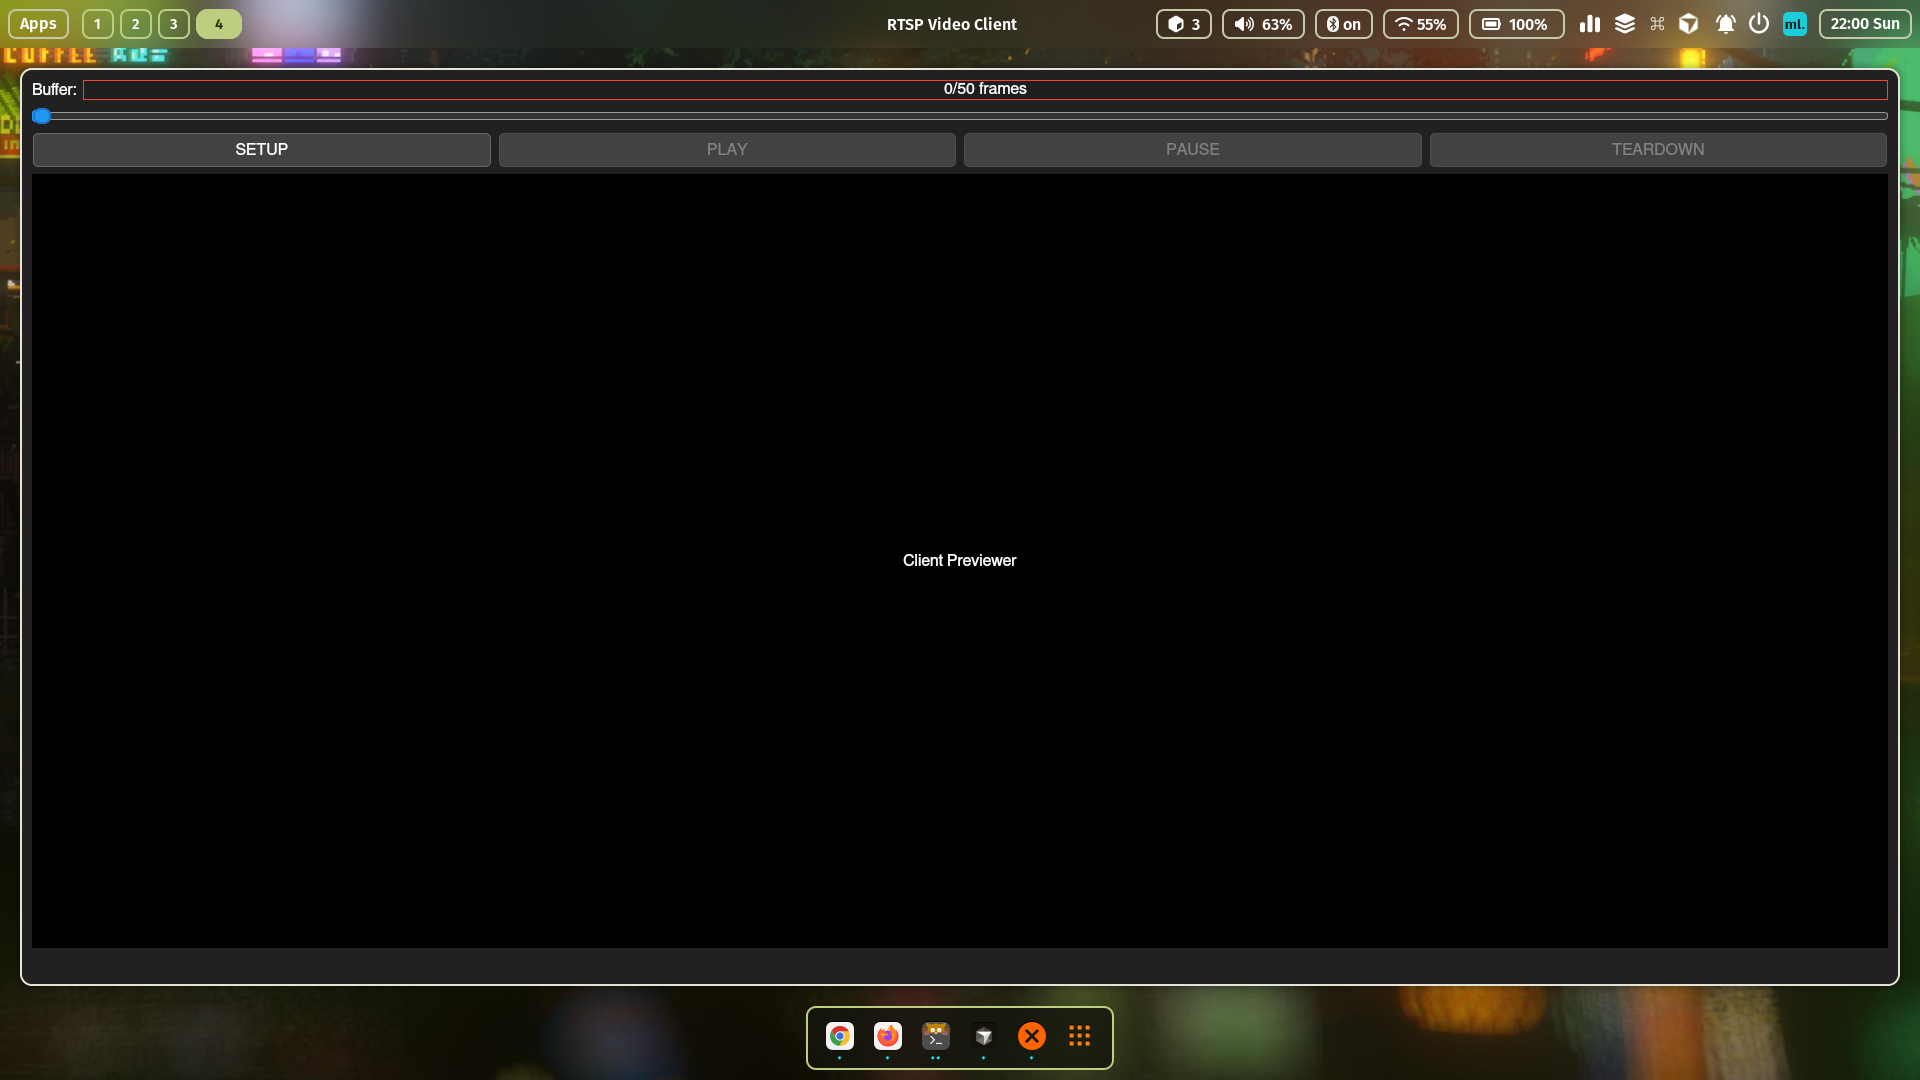
\includegraphics[width=0.9\textwidth]{images/client_ui_1.jpg}
    \caption{Giao diện của Client}
    \label{fig:client_ui}
\end{figure}

\begin{figure}[H]
    \centering
    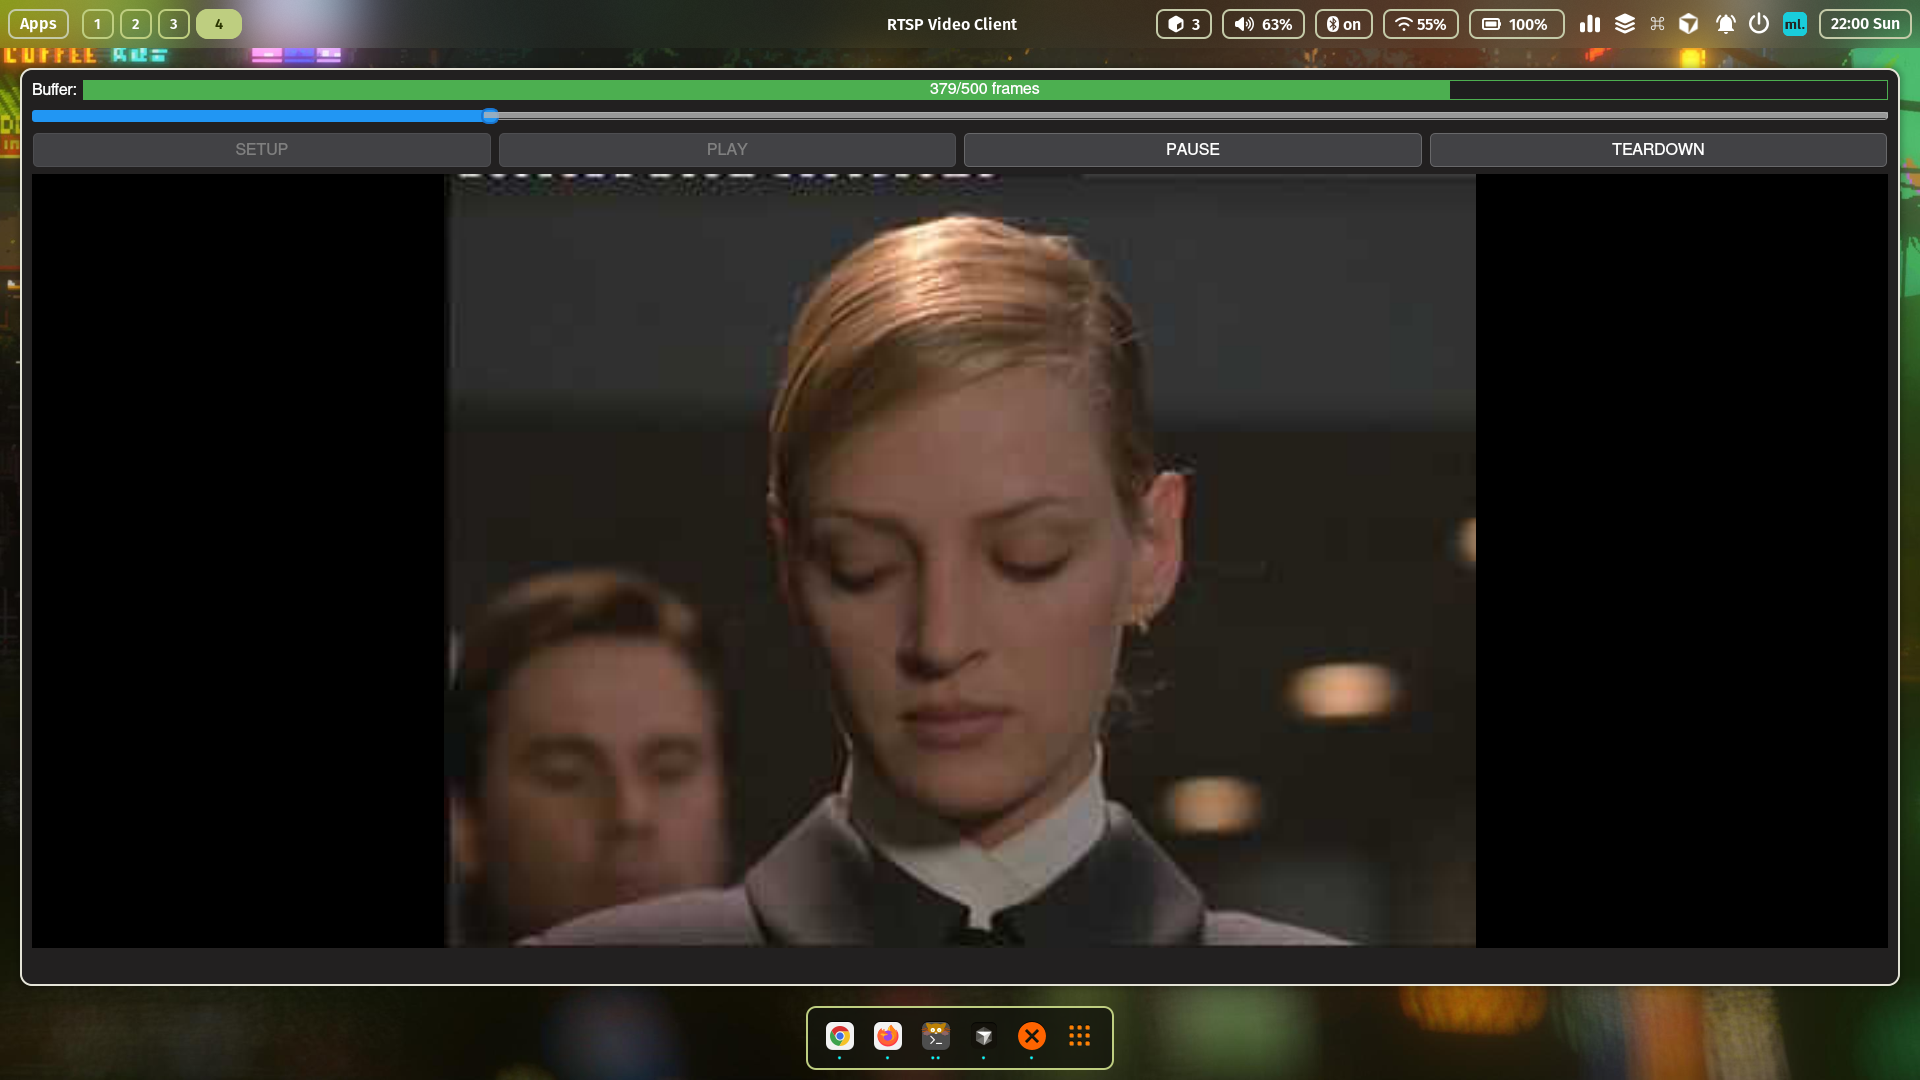
\includegraphics[width=0.9\textwidth]{images/client_ui_2.jpg}
    \caption{Giao diện của Client}
    \label{fig:client_ui}
\end{figure}

\section{Video Demo}
Dự án này được xây dựng có thể phù hợp với đa nền tảng khác nhau và đây là các video demo dự án từ đầu

\paragraph*{Windows}: Xem tại \url{https://youtu.be/yzEE6nu5VPk}

\paragraph*{Linux/MacOS}: Xem tại \url{https://youtu.be/vO6-jbP4yDU}